% Created 2024-09-13 Fri 20:28
% Intended LaTeX compiler: pdflatex
\documentclass[letterpaper, 12pt]{article}
\usepackage[utf8]{inputenc}
\usepackage[T1]{fontenc}
\usepackage{graphicx}
\usepackage{longtable}
\usepackage{wrapfig}
\usepackage{rotating}
\usepackage[normalem]{ulem}
\usepackage{amsmath}
\usepackage{amssymb}
\usepackage{capt-of}
\usepackage{hyperref}
\usepackage{minted}
\usepackage{xcolor}
\usepackage{hyperref}
\usepackage{tocloft}
\usepackage{minted}
\usemintedstyle{manni}
\usepackage{pdfpages}
\usepackage{fancyhdr}
\usepackage{graphicx}
\usepackage[top=1.4in, left=0.5in, right=0.5in, bottom=0.8in]{geometry}
\usepackage[T1]{fontenc}
\usepackage{helvet}
\pagestyle{fancy}
\renewcommand{\headrulewidth}{0pt}
\renewcommand{\footrulewidth}{0pt}
\setlength{\parindent}{0em}
\setlength{\parskip}{1em}
\usepackage{hyperref}
\usepackage {color}
\usepackage {tabularray}
\usepackage{xcolor}
\hypersetup{
colorlinks=true,
linkcolor=blue,
filecolor=magenta,
urlcolor=cyan,
citecolor=green,
pdfborder={0 0 0}
}
\usepackage[most]{tcolorbox}
\author{Hilduara Abreu}
\date{2024-09-05}
\title{School Year 2024-25 | Principal Message June 2024}
\hypersetup{
 pdfauthor={Hilduara Abreu},
 pdftitle={School Year 2024-25 | Principal Message June 2024},
 pdfkeywords={},
 pdfsubject={},
 pdfcreator={Emacs 29.4 (Org mode 9.6.15)}, 
 pdflang={English}}
\begin{document}

\fancyfoot[C]{\setlength{\unitlength}{1in}\begin{picture}(5,0)\put(-1.8,-0.5){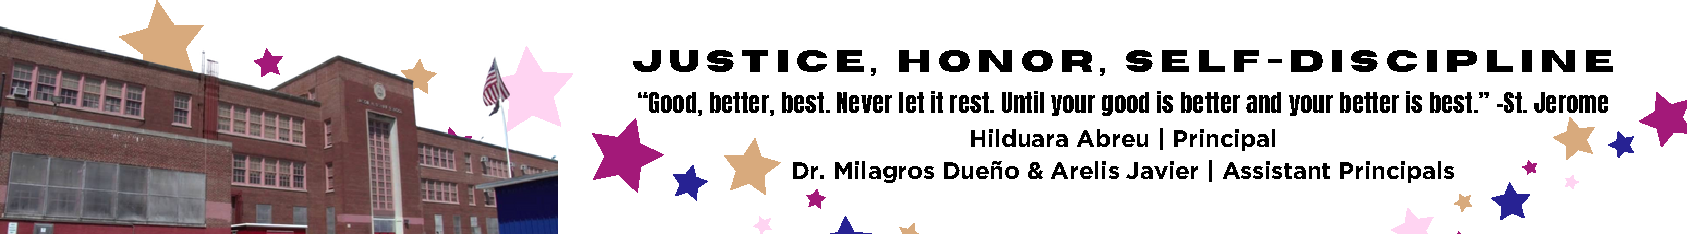
\includegraphics[width=8.8in,height=1.3in]{logo-1}}\end{picture}}
\fancyhead[C]{\setlength{\unitlength}{1in}\begin{picture}(5,0)\put(-1.9,-0.5){
\includegraphics[width=8.9in,height=1.3in]{logo-2}}\end{picture}}
\fancyhead[R]{\thepage}
\pagenumbering{gobble}

\begin{document}
\newpage
\vspace*{-0.5cm}
\textbf{Subject: Welcome to the 2024-2025 School Year}!

Dear PS 192 Community,

It is with great excitement and hope that we welcome all students, families, and staff to the start of the 2024-2025 academic year. This year marks the beginning of a new chapter filled with opportunities for growth, learning, and community building. At PS 192, we are proud to be ranked among the top schools in our district based on the latest state test results. This accomplishment is a testament to our collective hard work and dedication.

As we embark on this new journey, we are committed to excellence and driven by our core values of Justice, Honor, and Self-Discipline. These principles will guide us through each moment of learning and growth. I encourage everyone to take full advantage of the strong partnerships we continue to build. Be sure to mark your calendars for September 12, when we will hold our Parent-Teacher Conferences, a valuable time to connect with your child's educators. Additionally, on September 20, we invite you to join me for Coffee With The Principal, where we can come together to share ideas, concerns, and aspirations for the school year.

September also brings a time of celebration as we observe Hispanic Heritage Month, which begins on September 15. This is a wonderful opportunity for our school community to honor and celebrate the rich cultural history and contributions of the Hispanic community.

Our success is shared, and together we will accomplish even more this year. Let us enter this new academic year with hope, determination, and a strong commitment to ensuring every student thrives. I look forward to seeing the growth and achievements that we will celebrate together.

Wishing you all a fantastic year ahead!

With Justice, Honor, and Self-discipline,


\includegraphics[width=0.2\textwidth]{hil_signature}

\textbf{Hilduara Abreu, Principal}

\textbf{The school of Joyful Learning!}

\href{www.ps192.org}{www.ps192.org}
\end{document}
